% Options for packages loaded elsewhere
\PassOptionsToPackage{unicode}{hyperref}
\PassOptionsToPackage{hyphens}{url}
%
\documentclass[
]{book}
\usepackage{amsmath,amssymb}
\usepackage{lmodern}
\usepackage{iftex}
\ifPDFTeX
  \usepackage[T1]{fontenc}
  \usepackage[utf8]{inputenc}
  \usepackage{textcomp} % provide euro and other symbols
\else % if luatex or xetex
  \usepackage{unicode-math}
  \defaultfontfeatures{Scale=MatchLowercase}
  \defaultfontfeatures[\rmfamily]{Ligatures=TeX,Scale=1}
\fi
% Use upquote if available, for straight quotes in verbatim environments
\IfFileExists{upquote.sty}{\usepackage{upquote}}{}
\IfFileExists{microtype.sty}{% use microtype if available
  \usepackage[]{microtype}
  \UseMicrotypeSet[protrusion]{basicmath} % disable protrusion for tt fonts
}{}
\makeatletter
\@ifundefined{KOMAClassName}{% if non-KOMA class
  \IfFileExists{parskip.sty}{%
    \usepackage{parskip}
  }{% else
    \setlength{\parindent}{0pt}
    \setlength{\parskip}{6pt plus 2pt minus 1pt}}
}{% if KOMA class
  \KOMAoptions{parskip=half}}
\makeatother
\usepackage{xcolor}
\usepackage{listings}
\newcommand{\passthrough}[1]{#1}
\lstset{defaultdialect=[5.3]Lua}
\lstset{defaultdialect=[x86masm]Assembler}
\usepackage{longtable,booktabs,array}
\usepackage{calc} % for calculating minipage widths
% Correct order of tables after \paragraph or \subparagraph
\usepackage{etoolbox}
\makeatletter
\patchcmd\longtable{\par}{\if@noskipsec\mbox{}\fi\par}{}{}
\makeatother
% Allow footnotes in longtable head/foot
\IfFileExists{footnotehyper.sty}{\usepackage{footnotehyper}}{\usepackage{footnote}}
\makesavenoteenv{longtable}
\usepackage{graphicx}
\makeatletter
\def\maxwidth{\ifdim\Gin@nat@width>\linewidth\linewidth\else\Gin@nat@width\fi}
\def\maxheight{\ifdim\Gin@nat@height>\textheight\textheight\else\Gin@nat@height\fi}
\makeatother
% Scale images if necessary, so that they will not overflow the page
% margins by default, and it is still possible to overwrite the defaults
% using explicit options in \includegraphics[width, height, ...]{}
\setkeys{Gin}{width=\maxwidth,height=\maxheight,keepaspectratio}
% Set default figure placement to htbp
\makeatletter
\def\fps@figure{htbp}
\makeatother
\setlength{\emergencystretch}{3em} % prevent overfull lines
\providecommand{\tightlist}{%
  \setlength{\itemsep}{0pt}\setlength{\parskip}{0pt}}
\setcounter{secnumdepth}{5}
\lstset{
  breaklines=true
}
\usepackage{booktabs}
\usepackage{longtable}
\usepackage{array}
\usepackage{multirow}
\usepackage{wrapfig}
\usepackage{float}
\usepackage{colortbl}
\usepackage{pdflscape}
\usepackage{tabu}
\usepackage{threeparttable}
\usepackage{threeparttablex}
\usepackage[normalem]{ulem}
\usepackage{makecell}
\usepackage{xcolor}
\ifLuaTeX
  \usepackage{selnolig}  % disable illegal ligatures
\fi
\usepackage[]{natbib}
\bibliographystyle{apalike}
\nocite{*}
\IfFileExists{bookmark.sty}{\usepackage{bookmark}}{\usepackage{hyperref}}
\IfFileExists{xurl.sty}{\usepackage{xurl}}{} % add URL line breaks if available
\urlstyle{same} % disable monospaced font for URLs
\hypersetup{
  pdftitle={Supplemental Material for `Using lineage age to augment search space exploration in lexicase selection'},
  pdfauthor={Karen Suzue, Charles Ofria, and Alexander Lalejini},
  hidelinks,
  pdfcreator={LaTeX via pandoc}}

\title{Supplemental Material for `Using lineage age to augment search space exploration in lexicase selection'}
\author{Karen Suzue, Charles Ofria, and Alexander Lalejini}
\date{2024-07-16}

\begin{document}
\maketitle

{
\setcounter{tocdepth}{1}
\tableofcontents
}
\hypertarget{introduction}{%
\chapter{Introduction}\label{introduction}}

This is not intended as a stand-alone document, but as a companion to our manuscript.

\hypertarget{about-our-supplemental-material}{%
\section{About our supplemental material}\label{about-our-supplemental-material}}

As you may have noticed (unless you're reading a pdf version of this), our supplemental material is hosted using \href{https://pages.github.com/}{GitHub pages}.
We compiled our data analyses and supplemental documentation into this nifty web-accessible book using \href{https://bookdown.org}{bookdown}.

The source code/configuration files for this supplemental material can be found in \href{https://github.com/amlalejini/age-based-lex}{this GitHub repository}.

Our supplemental material includes the following:

\begin{itemize}
\tightlist
\item
  GP instruction set (Section \ref{signalgp-instruction-set})
\item
  GP data analysis + statistics (Section \ref{program-synthesis-experiments})
\end{itemize}

\hypertarget{contributing-authors}{%
\section{Contributing authors}\label{contributing-authors}}

\begin{itemize}
\tightlist
\item
  Karen Suzue
\item
  Charles Ofria
\item
  Alexander Lalejini
\end{itemize}

\hypertarget{signalgp-instruction-set}{%
\chapter{SignalGP instruction set}\label{signalgp-instruction-set}}

Below, we document the instruction set used in our GP system for our experiments.

Abbreviations:

\begin{itemize}
\tightlist
\item
  EOP: End of program
\item
  Reg: local register

  \begin{itemize}
  \tightlist
  \item
    Reg{[}0{]} indicates the value at the register specified by an instruction's first \emph{argument}, Reg{[}1{]} indicates the value at the register specified by an instruction's second argument, and Reg{[}2{]} indicates the value at the register specified by the instruction's third argument.
  \item
    Reg{[}0{]}, Reg{[}1{]}, \emph{etc}: Register 0, Register 1, \emph{etc.}
  \end{itemize}
\item
  Input: input buffer

  \begin{itemize}
  \tightlist
  \item
    Follows same scheme as Reg
  \end{itemize}
\item
  Output: output buffer

  \begin{itemize}
  \tightlist
  \item
    Follows same scheme as Reg
  \end{itemize}
\item
  Global: global memory buffer

  \begin{itemize}
  \tightlist
  \item
    Follows same scheme as Reg
  \end{itemize}
\item
  Arg: Instruction argument

  \begin{itemize}
  \tightlist
  \item
    Arg{[}i{]} indicates the i'th instruction argument (an integer encoded in the genome)
  \item
    E.g., Arg{[}0{]} is an instruction's first argument
  \end{itemize}
\end{itemize}

Instructions that would produce undefined behavior (e.g., division by zero) are treated as no operations.

\hypertarget{default-instructions}{%
\section{Default Instructions}\label{default-instructions}}

I.e., instructions used across all diagnostic tasks.

\begin{longtable}[]{@{}
  >{\raggedright\arraybackslash}p{(\columnwidth - 4\tabcolsep) * \real{0.3077}}
  >{\centering\arraybackslash}p{(\columnwidth - 4\tabcolsep) * \real{0.3846}}
  >{\raggedright\arraybackslash}p{(\columnwidth - 4\tabcolsep) * \real{0.3077}}@{}}
\toprule()
\begin{minipage}[b]{\linewidth}\raggedright
Instruction
\end{minipage} & \begin{minipage}[b]{\linewidth}\centering
Arguments Used
\end{minipage} & \begin{minipage}[b]{\linewidth}\raggedright
Description
\end{minipage} \\
\midrule()
\endhead
\passthrough{\lstinline!Nop!} & 0 & No operation \\
\passthrough{\lstinline!Not!} & 1 & Reg{[}0{]} = !Reg{[}0{]} \\
\passthrough{\lstinline!Inc!} & 1 & Reg{[}0{]} = Reg{[}0{]} + 1 \\
\passthrough{\lstinline!Dec!} & 1 & Reg{[}0{]} = Reg{[}0{]} - 1 \\
\passthrough{\lstinline!Add!} & 3 & Reg{[}0{]} = Reg{[}1{]} + Reg{[}2{]} \\
\passthrough{\lstinline!Sub!} & 3 & Reg{[}0{]} = Reg{[}1{]} - Reg{[}2{]} \\
\passthrough{\lstinline!Mult!} & 3 & Reg{[}0{]} = Reg{[}1{]} * Reg{[}2{]} \\
\passthrough{\lstinline!Div!} & 3 & Reg{[}0{]} = Reg{[}1{]} / Reg{[}2{]} \\
\passthrough{\lstinline!Mod!} & 3 & Reg{[}0{]} = Reg{[}1{]} \% Reg{[}2{]} \\
\passthrough{\lstinline!Nand!} & 2 & Reg{[}0{]} = !(R1g{[}0{]} \& Reg{[}2{]}) \\
\passthrough{\lstinline!TestEqu!} & 3 & Reg{[}0{]} = Reg{[}1{]} == Reg{[}2{]} \\
\passthrough{\lstinline!TestNEqu!} & 3 & Reg{[}0{]} = Reg{[}1{]} != Reg{[}2{]} \\
\passthrough{\lstinline!TestLess!} & 3 & Reg{[}0{]} = Reg{[}1{]} \textless{} Reg{[}2{]} \\
\passthrough{\lstinline!TestLessEqu!} & 3 & Reg{[}0{]} = Reg{[}1{]} \textless= Reg{[}2{]} \\
\passthrough{\lstinline!TestGreater!} & 3 & Reg{[}0{]} = Reg{[}1{]} \textgreater{} Reg{[}2{]} \\
\passthrough{\lstinline!TestGreaterEqu!} & 3 & Reg{[}0{]} = Reg{[}1{]} \textgreater= Reg{[}2{]} \\
\passthrough{\lstinline!SetMem!} & 2 & Reg{[}0{]} = Arg{[}1{]} \\
\passthrough{\lstinline!Terminal!} & 1 & Reg{[}0{]} = double value encoded by instruction tag \\
\passthrough{\lstinline!CopyMem!} & 2 & Reg{[}0{]} = Reg{[}1{]} \\
\passthrough{\lstinline!SwapMem!} & 2 & Swap(Reg{[}0{]}, Reg{[}1{]}) \\
\passthrough{\lstinline!InputToWorking!} & 2 & Reg{[}0{]} = Input{[}1{]} \\
\passthrough{\lstinline!WorkingToOutput!} & 2 & Output{[}1{]} = Reg{[}0{]} \\
\passthrough{\lstinline!If!} & 1 & If Reg{[}0{]} != 0, proceed. Otherwise skip to the next \passthrough{\lstinline!Close!} or EOP. \\
\passthrough{\lstinline!While!} & 1 & While Reg{[}0{]} != 0, loop. Otherwise skip to next \passthrough{\lstinline!Close!} or EOP. \\
\passthrough{\lstinline!Close!} & 0 & Indicate the end of a control block of code (e.g., loop, if). \\
\passthrough{\lstinline!Break!} & 0 & Break out of current control flow (e.g., loop). \\
\passthrough{\lstinline!Call!} & 0 & Call a function, using this instruction's tag to determine which function is called. \\
\passthrough{\lstinline!Routine!} & 0 & Same as call, but local memory is shared. Sort of like a jump that will jump back when the routine ends. \\
\passthrough{\lstinline!Return!} & 0 & Return from the current function call. \\
\passthrough{\lstinline!WorkingToGlobal!} & 2 & Global{[}1{]} = Reg{[}0{]} \\
\passthrough{\lstinline!GlobalToWorking!} & 2 & Reg{[}1{]} = Global{[}0{]} \\
\passthrough{\lstinline!FullGlobalToWorking!} & 0 & Copy entire global memory buffer into working memory buffer \\
\passthrough{\lstinline!FullWorkingToGlobal!} & 0 & Copy entire working memory buffer into global memory buffer \\
\bottomrule()
\end{longtable}

Note that \passthrough{\lstinline!Nand!} performs a bitwise operation.

\hypertarget{problem-specific-instructions}{%
\section{Problem-specific instructions}\label{problem-specific-instructions}}

Each problem has problem-specific instructions for producing output.

\hypertarget{bouncing-balls}{%
\subsection{Bouncing Balls}\label{bouncing-balls}}

\begin{itemize}
\tightlist
\item
  SubmitOutput
\end{itemize}

\hypertarget{dice-game}{%
\subsection{Dice Game}\label{dice-game}}

\begin{itemize}
\tightlist
\item
  SubmitOutput
\end{itemize}

\hypertarget{gcd}{%
\subsection{GCD}\label{gcd}}

\begin{itemize}
\tightlist
\item
  SubmitOutput
\end{itemize}

\hypertarget{grade}{%
\subsection{Grade}\label{grade}}

\begin{itemize}
\tightlist
\item
  SubmitA
\item
  SubmitB
\item
  SubmitC
\item
  SubmitD
\item
  SubmitF
\end{itemize}

\hypertarget{snow-day}{%
\subsection{Snow Day}\label{snow-day}}

\begin{itemize}
\tightlist
\item
  SubmitOutput
\end{itemize}

\hypertarget{program-synthesis-experiments}{%
\chapter{Program synthesis experiments}\label{program-synthesis-experiments}}

\begin{lstlisting}[language=R]
experiment_slug <- "2024-05-20-inj-int"

working_directory <- paste0(
  "experiments/",
  experiment_slug,
  "/analysis/"
)

if (exists("bookdown_wd_prefix")) {
  working_directory <- paste0(
    bookdown_wd_prefix,
    working_directory
  )
}
\end{lstlisting}

\hypertarget{dependencies}{%
\section{Dependencies}\label{dependencies}}

\begin{lstlisting}[language=R]
library(tidyverse)
\end{lstlisting}

\begin{lstlisting}
## Warning: package 'ggplot2' was built under R version 4.2.3
\end{lstlisting}

\begin{lstlisting}
## Warning: package 'dplyr' was built under R version 4.2.3
\end{lstlisting}

\begin{lstlisting}
## Warning: package 'stringr' was built under R version 4.2.3
\end{lstlisting}

\begin{lstlisting}
## -- Attaching core tidyverse packages -------------------------------------------------------------------------------------------------------------------------------------------------- tidyverse 2.0.0 --
## v dplyr     1.1.4     v readr     2.1.4
## v forcats   1.0.0     v stringr   1.5.1
## v ggplot2   3.5.1     v tibble    3.2.1
## v lubridate 1.9.3     v tidyr     1.3.0
## v purrr     1.0.2     
## -- Conflicts -------------------------------------------------------------------------------------------------------------------------------------------------------------------- tidyverse_conflicts() --
## x dplyr::filter() masks stats::filter()
## x dplyr::lag()    masks stats::lag()
## i Use the conflicted package (<http://conflicted.r-lib.org/>) to force all conflicts to become errors
\end{lstlisting}

\begin{lstlisting}[language=R]
library(cowplot)
\end{lstlisting}

\begin{lstlisting}
## Warning: package 'cowplot' was built under R version 4.2.3
\end{lstlisting}

\begin{lstlisting}
## 
## Attaching package: 'cowplot'
## 
## The following object is masked from 'package:lubridate':
## 
##     stamp
\end{lstlisting}

\begin{lstlisting}[language=R]
library(RColorBrewer)
library(khroma)
library(rstatix)
\end{lstlisting}

\begin{lstlisting}
## 
## Attaching package: 'rstatix'
## 
## The following object is masked from 'package:stats':
## 
##     filter
\end{lstlisting}

\begin{lstlisting}[language=R]
library(knitr)
library(kableExtra)
\end{lstlisting}

\begin{lstlisting}
## 
## Attaching package: 'kableExtra'
## 
## The following object is masked from 'package:dplyr':
## 
##     group_rows
\end{lstlisting}

\begin{lstlisting}[language=R]
source("https://gist.githubusercontent.com/benmarwick/2a1bb0133ff568cbe28d/raw/fb53bd97121f7f9ce947837ef1a4c65a73bffb3f/geom_flat_violin.R")
library(ggpattern)
\end{lstlisting}

\begin{lstlisting}[language=R]
print(version)
\end{lstlisting}

\begin{lstlisting}
##                _                           
## platform       aarch64-apple-darwin20      
## arch           aarch64                     
## os             darwin20                    
## system         aarch64, darwin20           
## status                                     
## major          4                           
## minor          2.1                         
## year           2022                        
## month          06                          
## day            23                          
## svn rev        82513                       
## language       R                           
## version.string R version 4.2.1 (2022-06-23)
## nickname       Funny-Looking Kid
\end{lstlisting}

\hypertarget{setup}{%
\section{Setup}\label{setup}}

\begin{lstlisting}[language=R]
# Configure our default graphing theme
theme_set(theme_cowplot())
# Create a directory to store plots
plot_directory <- paste0(working_directory, "plots/")
dir.create(plot_directory, showWarnings=FALSE)
\end{lstlisting}

\hypertarget{load-summary-data}{%
\subsection{Load summary data}\label{load-summary-data}}

\begin{lstlisting}[language=R]
summary_data_loc <- paste0(working_directory, "data/aggregate.csv")
summary_data <- read_csv(summary_data_loc)
\end{lstlisting}

\begin{lstlisting}
## Rows: 2700 Columns: 61
## -- Column specification ----------------------------------------------------------------------------------------------------------------------------------------------------------------------------------
## Delimiter: ","
## chr (11): ANCESTOR_FILE_PATH, EVAL_MODE, ORG_INJECTION_MODE, POP_INIT_MODE, ...
## dbl (50): AGE_LEX_AGE_ORDER_LIMIT, EVAL_CPU_CYCLES_PER_TEST, MAX_ACTIVE_THRE...
## 
## i Use `spec()` to retrieve the full column specification for this data.
## i Specify the column types or set `show_col_types = FALSE` to quiet this message.
\end{lstlisting}

\begin{lstlisting}[language=R]
summary_data <- summary_data %>%
  mutate(
    PROBLEM = as.factor(PROBLEM),
    SELECTION = as.factor(SELECTION),
    EVAL_MODE = as.factor(EVAL_MODE),
    NUM_COHORTS = as.factor(NUM_COHORTS),
    TEST_DOWNSAMPLE_RATE = as.factor(TEST_DOWNSAMPLE_RATE),
    AGE_LEX_AGE_ORDER_LIMIT = as.factor(AGE_LEX_AGE_ORDER_LIMIT),
    RECOMB_PER_FUNC_SEQ_RECOMB_RATE = as.factor(RECOMB_PER_FUNC_SEQ_RECOMB_RATE),
    ORG_INJECTION_COUNT = as.factor(ORG_INJECTION_COUNT),
    ORG_INJECTION_MODE = factor(
      ORG_INJECTION_MODE,
      levels = c(
        "none",
        "random",
        "recombine-random",
        "recombine-complement"
      )
    ),
    inject_cond = str_c(SELECTION, ORG_INJECTION_MODE, sep = "_"),
    ORG_INJECTION_INTERVAL = as.factor(ORG_INJECTION_INTERVAL),
    .keep = "all"
  ) %>%
  mutate(
    inject_cond = factor(
      inject_cond,
      levels = c(
        "age-lexicase_random",
        "lexicase_random",
        "lexicase_none"
      ),
      labels = c(
        "age-lex_inj-rand",
        "lex_inj-rand",
        "lex_inj-none"
      )
    )
  )

solution_counts <- summary_data %>%
  group_by(
    PROBLEM,
    SELECTION,
    AGE_LEX_AGE_ORDER_LIMIT,
    ORG_INJECTION_COUNT,
    ORG_INJECTION_MODE,
    ORG_INJECTION_INTERVAL,
    inject_cond
  ) %>%
  summarize(
    solution_count = sum(found_solution == "1"),
    replicates = n(),
    no_solution_count = n() - sum(found_solution == "1"),
    elite_from_injected = sum(elite_elite_age != update),
    sol_from_injected = sum(elite_elite_age != update & found_solution == "1")
  )
\end{lstlisting}

\begin{lstlisting}
## `summarise()` has grouped output by 'PROBLEM', 'SELECTION', 'AGE_LEX_AGE_ORDER_LIMIT', 'ORG_INJECTION_COUNT', 'ORG_INJECTION_MODE', 'ORG_INJECTION_INTERVAL'. You can override using the `.groups`
## argument.
\end{lstlisting}

\begin{lstlisting}[language=R]
# print(solution_counts, n=208)
solution_table <- kable(solution_counts) %>%
  kable_styling(latex_options = "striped", font_size = 25)
save_kable(solution_table, paste0(plot_directory, "solution_counts_table.pdf"))
solution_table
\end{lstlisting}

\begin{table}
\centering\begingroup\fontsize{25}{27}\selectfont

\begin{tabular}{l|l|l|l|l|l|l|r|r|r|r|r}
\hline
PROBLEM & SELECTION & AGE\_LEX\_AGE\_ORDER\_LIMIT & ORG\_INJECTION\_COUNT & ORG\_INJECTION\_MODE & ORG\_INJECTION\_INTERVAL & inject\_cond & solution\_count & replicates & no\_solution\_count & elite\_from\_injected & sol\_from\_injected\\
\hline
\cellcolor{gray!6}{bouncing-balls} & \cellcolor{gray!6}{age-lexicase} & \cellcolor{gray!6}{10} & \cellcolor{gray!6}{100} & \cellcolor{gray!6}{random} & \cellcolor{gray!6}{100} & \cellcolor{gray!6}{age-lex\_inj-rand} & \cellcolor{gray!6}{1} & \cellcolor{gray!6}{30} & \cellcolor{gray!6}{29} & \cellcolor{gray!6}{6} & \cellcolor{gray!6}{0}\\
\hline
bouncing-balls & age-lexicase & 10 & 100 & random & 500 & age-lex\_inj-rand & 4 & 30 & 26 & 8 & 0\\
\hline
\cellcolor{gray!6}{bouncing-balls} & \cellcolor{gray!6}{age-lexicase} & \cellcolor{gray!6}{10} & \cellcolor{gray!6}{100} & \cellcolor{gray!6}{random} & \cellcolor{gray!6}{1000} & \cellcolor{gray!6}{age-lex\_inj-rand} & \cellcolor{gray!6}{1} & \cellcolor{gray!6}{30} & \cellcolor{gray!6}{29} & \cellcolor{gray!6}{6} & \cellcolor{gray!6}{0}\\
\hline
bouncing-balls & age-lexicase & 20 & 100 & random & 100 & age-lex\_inj-rand & 0 & 30 & 30 & 3 & 0\\
\hline
\cellcolor{gray!6}{bouncing-balls} & \cellcolor{gray!6}{age-lexicase} & \cellcolor{gray!6}{20} & \cellcolor{gray!6}{100} & \cellcolor{gray!6}{random} & \cellcolor{gray!6}{500} & \cellcolor{gray!6}{age-lex\_inj-rand} & \cellcolor{gray!6}{1} & \cellcolor{gray!6}{30} & \cellcolor{gray!6}{29} & \cellcolor{gray!6}{3} & \cellcolor{gray!6}{0}\\
\hline
bouncing-balls & age-lexicase & 20 & 100 & random & 1000 & age-lex\_inj-rand & 0 & 30 & 30 & 3 & 0\\
\hline
\cellcolor{gray!6}{bouncing-balls} & \cellcolor{gray!6}{lexicase} & \cellcolor{gray!6}{10} & \cellcolor{gray!6}{100} & \cellcolor{gray!6}{none} & \cellcolor{gray!6}{100} & \cellcolor{gray!6}{lex\_inj-none} & \cellcolor{gray!6}{3} & \cellcolor{gray!6}{30} & \cellcolor{gray!6}{27} & \cellcolor{gray!6}{0} & \cellcolor{gray!6}{0}\\
\hline
bouncing-balls & lexicase & 10 & 100 & none & 500 & lex\_inj-none & 1 & 30 & 29 & 0 & 0\\
\hline
\cellcolor{gray!6}{bouncing-balls} & \cellcolor{gray!6}{lexicase} & \cellcolor{gray!6}{10} & \cellcolor{gray!6}{100} & \cellcolor{gray!6}{none} & \cellcolor{gray!6}{1000} & \cellcolor{gray!6}{lex\_inj-none} & \cellcolor{gray!6}{0} & \cellcolor{gray!6}{30} & \cellcolor{gray!6}{30} & \cellcolor{gray!6}{0} & \cellcolor{gray!6}{0}\\
\hline
bouncing-balls & lexicase & 10 & 100 & random & 100 & lex\_inj-rand & 0 & 30 & 30 & 0 & 0\\
\hline
\cellcolor{gray!6}{bouncing-balls} & \cellcolor{gray!6}{lexicase} & \cellcolor{gray!6}{10} & \cellcolor{gray!6}{100} & \cellcolor{gray!6}{random} & \cellcolor{gray!6}{500} & \cellcolor{gray!6}{lex\_inj-rand} & \cellcolor{gray!6}{1} & \cellcolor{gray!6}{30} & \cellcolor{gray!6}{29} & \cellcolor{gray!6}{0} & \cellcolor{gray!6}{0}\\
\hline
bouncing-balls & lexicase & 10 & 100 & random & 1000 & lex\_inj-rand & 2 & 30 & 28 & 0 & 0\\
\hline
\cellcolor{gray!6}{bouncing-balls} & \cellcolor{gray!6}{lexicase} & \cellcolor{gray!6}{20} & \cellcolor{gray!6}{100} & \cellcolor{gray!6}{none} & \cellcolor{gray!6}{100} & \cellcolor{gray!6}{lex\_inj-none} & \cellcolor{gray!6}{1} & \cellcolor{gray!6}{30} & \cellcolor{gray!6}{29} & \cellcolor{gray!6}{0} & \cellcolor{gray!6}{0}\\
\hline
bouncing-balls & lexicase & 20 & 100 & none & 500 & lex\_inj-none & 3 & 30 & 27 & 0 & 0\\
\hline
\cellcolor{gray!6}{bouncing-balls} & \cellcolor{gray!6}{lexicase} & \cellcolor{gray!6}{20} & \cellcolor{gray!6}{100} & \cellcolor{gray!6}{none} & \cellcolor{gray!6}{1000} & \cellcolor{gray!6}{lex\_inj-none} & \cellcolor{gray!6}{0} & \cellcolor{gray!6}{30} & \cellcolor{gray!6}{30} & \cellcolor{gray!6}{0} & \cellcolor{gray!6}{0}\\
\hline
bouncing-balls & lexicase & 20 & 100 & random & 100 & lex\_inj-rand & 1 & 30 & 29 & 0 & 0\\
\hline
\cellcolor{gray!6}{bouncing-balls} & \cellcolor{gray!6}{lexicase} & \cellcolor{gray!6}{20} & \cellcolor{gray!6}{100} & \cellcolor{gray!6}{random} & \cellcolor{gray!6}{500} & \cellcolor{gray!6}{lex\_inj-rand} & \cellcolor{gray!6}{0} & \cellcolor{gray!6}{30} & \cellcolor{gray!6}{30} & \cellcolor{gray!6}{0} & \cellcolor{gray!6}{0}\\
\hline
bouncing-balls & lexicase & 20 & 100 & random & 1000 & lex\_inj-rand & 1 & 30 & 29 & 0 & 0\\
\hline
\cellcolor{gray!6}{dice-game} & \cellcolor{gray!6}{age-lexicase} & \cellcolor{gray!6}{10} & \cellcolor{gray!6}{100} & \cellcolor{gray!6}{random} & \cellcolor{gray!6}{100} & \cellcolor{gray!6}{age-lex\_inj-rand} & \cellcolor{gray!6}{20} & \cellcolor{gray!6}{30} & \cellcolor{gray!6}{10} & \cellcolor{gray!6}{0} & \cellcolor{gray!6}{0}\\
\hline
dice-game & age-lexicase & 10 & 100 & random & 500 & age-lex\_inj-rand & 10 & 30 & 20 & 4 & 1\\
\hline
\cellcolor{gray!6}{dice-game} & \cellcolor{gray!6}{age-lexicase} & \cellcolor{gray!6}{10} & \cellcolor{gray!6}{100} & \cellcolor{gray!6}{random} & \cellcolor{gray!6}{1000} & \cellcolor{gray!6}{age-lex\_inj-rand} & \cellcolor{gray!6}{15} & \cellcolor{gray!6}{30} & \cellcolor{gray!6}{15} & \cellcolor{gray!6}{9} & \cellcolor{gray!6}{4}\\
\hline
dice-game & age-lexicase & 20 & 100 & random & 100 & age-lex\_inj-rand & 17 & 30 & 13 & 0 & 0\\
\hline
\cellcolor{gray!6}{dice-game} & \cellcolor{gray!6}{age-lexicase} & \cellcolor{gray!6}{20} & \cellcolor{gray!6}{100} & \cellcolor{gray!6}{random} & \cellcolor{gray!6}{500} & \cellcolor{gray!6}{age-lex\_inj-rand} & \cellcolor{gray!6}{13} & \cellcolor{gray!6}{30} & \cellcolor{gray!6}{17} & \cellcolor{gray!6}{1} & \cellcolor{gray!6}{0}\\
\hline
dice-game & age-lexicase & 20 & 100 & random & 1000 & age-lex\_inj-rand & 13 & 30 & 17 & 0 & 0\\
\hline
\cellcolor{gray!6}{dice-game} & \cellcolor{gray!6}{lexicase} & \cellcolor{gray!6}{10} & \cellcolor{gray!6}{100} & \cellcolor{gray!6}{none} & \cellcolor{gray!6}{100} & \cellcolor{gray!6}{lex\_inj-none} & \cellcolor{gray!6}{15} & \cellcolor{gray!6}{30} & \cellcolor{gray!6}{15} & \cellcolor{gray!6}{0} & \cellcolor{gray!6}{0}\\
\hline
dice-game & lexicase & 10 & 100 & none & 500 & lex\_inj-none & 16 & 30 & 14 & 0 & 0\\
\hline
\cellcolor{gray!6}{dice-game} & \cellcolor{gray!6}{lexicase} & \cellcolor{gray!6}{10} & \cellcolor{gray!6}{100} & \cellcolor{gray!6}{none} & \cellcolor{gray!6}{1000} & \cellcolor{gray!6}{lex\_inj-none} & \cellcolor{gray!6}{14} & \cellcolor{gray!6}{30} & \cellcolor{gray!6}{16} & \cellcolor{gray!6}{0} & \cellcolor{gray!6}{0}\\
\hline
dice-game & lexicase & 10 & 100 & random & 100 & lex\_inj-rand & 14 & 30 & 16 & 0 & 0\\
\hline
\cellcolor{gray!6}{dice-game} & \cellcolor{gray!6}{lexicase} & \cellcolor{gray!6}{10} & \cellcolor{gray!6}{100} & \cellcolor{gray!6}{random} & \cellcolor{gray!6}{500} & \cellcolor{gray!6}{lex\_inj-rand} & \cellcolor{gray!6}{14} & \cellcolor{gray!6}{30} & \cellcolor{gray!6}{16} & \cellcolor{gray!6}{0} & \cellcolor{gray!6}{0}\\
\hline
dice-game & lexicase & 10 & 100 & random & 1000 & lex\_inj-rand & 17 & 30 & 13 & 0 & 0\\
\hline
\cellcolor{gray!6}{dice-game} & \cellcolor{gray!6}{lexicase} & \cellcolor{gray!6}{20} & \cellcolor{gray!6}{100} & \cellcolor{gray!6}{none} & \cellcolor{gray!6}{100} & \cellcolor{gray!6}{lex\_inj-none} & \cellcolor{gray!6}{10} & \cellcolor{gray!6}{30} & \cellcolor{gray!6}{20} & \cellcolor{gray!6}{0} & \cellcolor{gray!6}{0}\\
\hline
dice-game & lexicase & 20 & 100 & none & 500 & lex\_inj-none & 9 & 30 & 21 & 0 & 0\\
\hline
\cellcolor{gray!6}{dice-game} & \cellcolor{gray!6}{lexicase} & \cellcolor{gray!6}{20} & \cellcolor{gray!6}{100} & \cellcolor{gray!6}{none} & \cellcolor{gray!6}{1000} & \cellcolor{gray!6}{lex\_inj-none} & \cellcolor{gray!6}{14} & \cellcolor{gray!6}{30} & \cellcolor{gray!6}{16} & \cellcolor{gray!6}{0} & \cellcolor{gray!6}{0}\\
\hline
dice-game & lexicase & 20 & 100 & random & 100 & lex\_inj-rand & 15 & 30 & 15 & 0 & 0\\
\hline
\cellcolor{gray!6}{dice-game} & \cellcolor{gray!6}{lexicase} & \cellcolor{gray!6}{20} & \cellcolor{gray!6}{100} & \cellcolor{gray!6}{random} & \cellcolor{gray!6}{500} & \cellcolor{gray!6}{lex\_inj-rand} & \cellcolor{gray!6}{15} & \cellcolor{gray!6}{30} & \cellcolor{gray!6}{15} & \cellcolor{gray!6}{0} & \cellcolor{gray!6}{0}\\
\hline
dice-game & lexicase & 20 & 100 & random & 1000 & lex\_inj-rand & 9 & 30 & 21 & 0 & 0\\
\hline
\cellcolor{gray!6}{gcd} & \cellcolor{gray!6}{age-lexicase} & \cellcolor{gray!6}{10} & \cellcolor{gray!6}{100} & \cellcolor{gray!6}{random} & \cellcolor{gray!6}{100} & \cellcolor{gray!6}{age-lex\_inj-rand} & \cellcolor{gray!6}{19} & \cellcolor{gray!6}{30} & \cellcolor{gray!6}{11} & \cellcolor{gray!6}{29} & \cellcolor{gray!6}{18}\\
\hline
gcd & age-lexicase & 10 & 100 & random & 500 & age-lex\_inj-rand & 27 & 30 & 3 & 21 & 18\\
\hline
\cellcolor{gray!6}{gcd} & \cellcolor{gray!6}{age-lexicase} & \cellcolor{gray!6}{10} & \cellcolor{gray!6}{100} & \cellcolor{gray!6}{random} & \cellcolor{gray!6}{1000} & \cellcolor{gray!6}{age-lex\_inj-rand} & \cellcolor{gray!6}{24} & \cellcolor{gray!6}{30} & \cellcolor{gray!6}{6} & \cellcolor{gray!6}{17} & \cellcolor{gray!6}{13}\\
\hline
gcd & age-lexicase & 20 & 100 & random & 100 & age-lex\_inj-rand & 19 & 30 & 11 & 17 & 11\\
\hline
\cellcolor{gray!6}{gcd} & \cellcolor{gray!6}{age-lexicase} & \cellcolor{gray!6}{20} & \cellcolor{gray!6}{100} & \cellcolor{gray!6}{random} & \cellcolor{gray!6}{500} & \cellcolor{gray!6}{age-lex\_inj-rand} & \cellcolor{gray!6}{20} & \cellcolor{gray!6}{30} & \cellcolor{gray!6}{10} & \cellcolor{gray!6}{7} & \cellcolor{gray!6}{5}\\
\hline
gcd & age-lexicase & 20 & 100 & random & 1000 & age-lex\_inj-rand & 24 & 30 & 6 & 6 & 5\\
\hline
\cellcolor{gray!6}{gcd} & \cellcolor{gray!6}{lexicase} & \cellcolor{gray!6}{10} & \cellcolor{gray!6}{100} & \cellcolor{gray!6}{none} & \cellcolor{gray!6}{100} & \cellcolor{gray!6}{lex\_inj-none} & \cellcolor{gray!6}{18} & \cellcolor{gray!6}{30} & \cellcolor{gray!6}{12} & \cellcolor{gray!6}{0} & \cellcolor{gray!6}{0}\\
\hline
gcd & lexicase & 10 & 100 & none & 500 & lex\_inj-none & 19 & 30 & 11 & 0 & 0\\
\hline
\cellcolor{gray!6}{gcd} & \cellcolor{gray!6}{lexicase} & \cellcolor{gray!6}{10} & \cellcolor{gray!6}{100} & \cellcolor{gray!6}{none} & \cellcolor{gray!6}{1000} & \cellcolor{gray!6}{lex\_inj-none} & \cellcolor{gray!6}{21} & \cellcolor{gray!6}{30} & \cellcolor{gray!6}{9} & \cellcolor{gray!6}{0} & \cellcolor{gray!6}{0}\\
\hline
gcd & lexicase & 10 & 100 & random & 100 & lex\_inj-rand & 16 & 30 & 14 & 0 & 0\\
\hline
\cellcolor{gray!6}{gcd} & \cellcolor{gray!6}{lexicase} & \cellcolor{gray!6}{10} & \cellcolor{gray!6}{100} & \cellcolor{gray!6}{random} & \cellcolor{gray!6}{500} & \cellcolor{gray!6}{lex\_inj-rand} & \cellcolor{gray!6}{22} & \cellcolor{gray!6}{30} & \cellcolor{gray!6}{8} & \cellcolor{gray!6}{0} & \cellcolor{gray!6}{0}\\
\hline
gcd & lexicase & 10 & 100 & random & 1000 & lex\_inj-rand & 22 & 30 & 8 & 0 & 0\\
\hline
\cellcolor{gray!6}{gcd} & \cellcolor{gray!6}{lexicase} & \cellcolor{gray!6}{20} & \cellcolor{gray!6}{100} & \cellcolor{gray!6}{none} & \cellcolor{gray!6}{100} & \cellcolor{gray!6}{lex\_inj-none} & \cellcolor{gray!6}{22} & \cellcolor{gray!6}{30} & \cellcolor{gray!6}{8} & \cellcolor{gray!6}{0} & \cellcolor{gray!6}{0}\\
\hline
gcd & lexicase & 20 & 100 & none & 500 & lex\_inj-none & 22 & 30 & 8 & 0 & 0\\
\hline
\cellcolor{gray!6}{gcd} & \cellcolor{gray!6}{lexicase} & \cellcolor{gray!6}{20} & \cellcolor{gray!6}{100} & \cellcolor{gray!6}{none} & \cellcolor{gray!6}{1000} & \cellcolor{gray!6}{lex\_inj-none} & \cellcolor{gray!6}{19} & \cellcolor{gray!6}{30} & \cellcolor{gray!6}{11} & \cellcolor{gray!6}{0} & \cellcolor{gray!6}{0}\\
\hline
gcd & lexicase & 20 & 100 & random & 100 & lex\_inj-rand & 17 & 30 & 13 & 0 & 0\\
\hline
\cellcolor{gray!6}{gcd} & \cellcolor{gray!6}{lexicase} & \cellcolor{gray!6}{20} & \cellcolor{gray!6}{100} & \cellcolor{gray!6}{random} & \cellcolor{gray!6}{500} & \cellcolor{gray!6}{lex\_inj-rand} & \cellcolor{gray!6}{17} & \cellcolor{gray!6}{30} & \cellcolor{gray!6}{13} & \cellcolor{gray!6}{0} & \cellcolor{gray!6}{0}\\
\hline
gcd & lexicase & 20 & 100 & random & 1000 & lex\_inj-rand & 20 & 30 & 10 & 0 & 0\\
\hline
\cellcolor{gray!6}{grade} & \cellcolor{gray!6}{age-lexicase} & \cellcolor{gray!6}{10} & \cellcolor{gray!6}{100} & \cellcolor{gray!6}{random} & \cellcolor{gray!6}{100} & \cellcolor{gray!6}{age-lex\_inj-rand} & \cellcolor{gray!6}{30} & \cellcolor{gray!6}{30} & \cellcolor{gray!6}{0} & \cellcolor{gray!6}{21} & \cellcolor{gray!6}{21}\\
\hline
grade & age-lexicase & 10 & 100 & random & 500 & age-lex\_inj-rand & 30 & 30 & 0 & 21 & 21\\
\hline
\cellcolor{gray!6}{grade} & \cellcolor{gray!6}{age-lexicase} & \cellcolor{gray!6}{10} & \cellcolor{gray!6}{100} & \cellcolor{gray!6}{random} & \cellcolor{gray!6}{1000} & \cellcolor{gray!6}{age-lex\_inj-rand} & \cellcolor{gray!6}{30} & \cellcolor{gray!6}{30} & \cellcolor{gray!6}{0} & \cellcolor{gray!6}{16} & \cellcolor{gray!6}{16}\\
\hline
grade & age-lexicase & 20 & 100 & random & 100 & age-lex\_inj-rand & 30 & 30 & 0 & 20 & 20\\
\hline
\cellcolor{gray!6}{grade} & \cellcolor{gray!6}{age-lexicase} & \cellcolor{gray!6}{20} & \cellcolor{gray!6}{100} & \cellcolor{gray!6}{random} & \cellcolor{gray!6}{500} & \cellcolor{gray!6}{age-lex\_inj-rand} & \cellcolor{gray!6}{30} & \cellcolor{gray!6}{30} & \cellcolor{gray!6}{0} & \cellcolor{gray!6}{12} & \cellcolor{gray!6}{12}\\
\hline
grade & age-lexicase & 20 & 100 & random & 1000 & age-lex\_inj-rand & 30 & 30 & 0 & 11 & 11\\
\hline
\cellcolor{gray!6}{grade} & \cellcolor{gray!6}{lexicase} & \cellcolor{gray!6}{10} & \cellcolor{gray!6}{100} & \cellcolor{gray!6}{none} & \cellcolor{gray!6}{100} & \cellcolor{gray!6}{lex\_inj-none} & \cellcolor{gray!6}{20} & \cellcolor{gray!6}{30} & \cellcolor{gray!6}{10} & \cellcolor{gray!6}{0} & \cellcolor{gray!6}{0}\\
\hline
grade & lexicase & 10 & 100 & none & 500 & lex\_inj-none & 24 & 30 & 6 & 0 & 0\\
\hline
\cellcolor{gray!6}{grade} & \cellcolor{gray!6}{lexicase} & \cellcolor{gray!6}{10} & \cellcolor{gray!6}{100} & \cellcolor{gray!6}{none} & \cellcolor{gray!6}{1000} & \cellcolor{gray!6}{lex\_inj-none} & \cellcolor{gray!6}{23} & \cellcolor{gray!6}{30} & \cellcolor{gray!6}{7} & \cellcolor{gray!6}{0} & \cellcolor{gray!6}{0}\\
\hline
grade & lexicase & 10 & 100 & random & 100 & lex\_inj-rand & 21 & 30 & 9 & 0 & 0\\
\hline
\cellcolor{gray!6}{grade} & \cellcolor{gray!6}{lexicase} & \cellcolor{gray!6}{10} & \cellcolor{gray!6}{100} & \cellcolor{gray!6}{random} & \cellcolor{gray!6}{500} & \cellcolor{gray!6}{lex\_inj-rand} & \cellcolor{gray!6}{23} & \cellcolor{gray!6}{30} & \cellcolor{gray!6}{7} & \cellcolor{gray!6}{0} & \cellcolor{gray!6}{0}\\
\hline
grade & lexicase & 10 & 100 & random & 1000 & lex\_inj-rand & 18 & 30 & 12 & 0 & 0\\
\hline
\cellcolor{gray!6}{grade} & \cellcolor{gray!6}{lexicase} & \cellcolor{gray!6}{20} & \cellcolor{gray!6}{100} & \cellcolor{gray!6}{none} & \cellcolor{gray!6}{100} & \cellcolor{gray!6}{lex\_inj-none} & \cellcolor{gray!6}{23} & \cellcolor{gray!6}{30} & \cellcolor{gray!6}{7} & \cellcolor{gray!6}{0} & \cellcolor{gray!6}{0}\\
\hline
grade & lexicase & 20 & 100 & none & 500 & lex\_inj-none & 21 & 30 & 9 & 0 & 0\\
\hline
\cellcolor{gray!6}{grade} & \cellcolor{gray!6}{lexicase} & \cellcolor{gray!6}{20} & \cellcolor{gray!6}{100} & \cellcolor{gray!6}{none} & \cellcolor{gray!6}{1000} & \cellcolor{gray!6}{lex\_inj-none} & \cellcolor{gray!6}{16} & \cellcolor{gray!6}{30} & \cellcolor{gray!6}{14} & \cellcolor{gray!6}{0} & \cellcolor{gray!6}{0}\\
\hline
grade & lexicase & 20 & 100 & random & 100 & lex\_inj-rand & 18 & 30 & 12 & 0 & 0\\
\hline
\cellcolor{gray!6}{grade} & \cellcolor{gray!6}{lexicase} & \cellcolor{gray!6}{20} & \cellcolor{gray!6}{100} & \cellcolor{gray!6}{random} & \cellcolor{gray!6}{500} & \cellcolor{gray!6}{lex\_inj-rand} & \cellcolor{gray!6}{24} & \cellcolor{gray!6}{30} & \cellcolor{gray!6}{6} & \cellcolor{gray!6}{0} & \cellcolor{gray!6}{0}\\
\hline
grade & lexicase & 20 & 100 & random & 1000 & lex\_inj-rand & 21 & 30 & 9 & 0 & 0\\
\hline
\cellcolor{gray!6}{snow-day} & \cellcolor{gray!6}{age-lexicase} & \cellcolor{gray!6}{10} & \cellcolor{gray!6}{100} & \cellcolor{gray!6}{random} & \cellcolor{gray!6}{100} & \cellcolor{gray!6}{age-lex\_inj-rand} & \cellcolor{gray!6}{0} & \cellcolor{gray!6}{30} & \cellcolor{gray!6}{30} & \cellcolor{gray!6}{9} & \cellcolor{gray!6}{0}\\
\hline
snow-day & age-lexicase & 10 & 100 & random & 500 & age-lex\_inj-rand & 0 & 30 & 30 & 7 & 0\\
\hline
\cellcolor{gray!6}{snow-day} & \cellcolor{gray!6}{age-lexicase} & \cellcolor{gray!6}{10} & \cellcolor{gray!6}{100} & \cellcolor{gray!6}{random} & \cellcolor{gray!6}{1000} & \cellcolor{gray!6}{age-lex\_inj-rand} & \cellcolor{gray!6}{2} & \cellcolor{gray!6}{30} & \cellcolor{gray!6}{28} & \cellcolor{gray!6}{9} & \cellcolor{gray!6}{0}\\
\hline
snow-day & age-lexicase & 20 & 100 & random & 100 & age-lex\_inj-rand & 2 & 30 & 28 & 2 & 1\\
\hline
\cellcolor{gray!6}{snow-day} & \cellcolor{gray!6}{age-lexicase} & \cellcolor{gray!6}{20} & \cellcolor{gray!6}{100} & \cellcolor{gray!6}{random} & \cellcolor{gray!6}{500} & \cellcolor{gray!6}{age-lex\_inj-rand} & \cellcolor{gray!6}{1} & \cellcolor{gray!6}{30} & \cellcolor{gray!6}{29} & \cellcolor{gray!6}{4} & \cellcolor{gray!6}{0}\\
\hline
snow-day & age-lexicase & 20 & 100 & random & 1000 & age-lex\_inj-rand & 1 & 30 & 29 & 2 & 0\\
\hline
\cellcolor{gray!6}{snow-day} & \cellcolor{gray!6}{lexicase} & \cellcolor{gray!6}{10} & \cellcolor{gray!6}{100} & \cellcolor{gray!6}{none} & \cellcolor{gray!6}{100} & \cellcolor{gray!6}{lex\_inj-none} & \cellcolor{gray!6}{0} & \cellcolor{gray!6}{30} & \cellcolor{gray!6}{30} & \cellcolor{gray!6}{0} & \cellcolor{gray!6}{0}\\
\hline
snow-day & lexicase & 10 & 100 & none & 500 & lex\_inj-none & 0 & 30 & 30 & 0 & 0\\
\hline
\cellcolor{gray!6}{snow-day} & \cellcolor{gray!6}{lexicase} & \cellcolor{gray!6}{10} & \cellcolor{gray!6}{100} & \cellcolor{gray!6}{none} & \cellcolor{gray!6}{1000} & \cellcolor{gray!6}{lex\_inj-none} & \cellcolor{gray!6}{0} & \cellcolor{gray!6}{30} & \cellcolor{gray!6}{30} & \cellcolor{gray!6}{0} & \cellcolor{gray!6}{0}\\
\hline
snow-day & lexicase & 10 & 100 & random & 100 & lex\_inj-rand & 1 & 30 & 29 & 0 & 0\\
\hline
\cellcolor{gray!6}{snow-day} & \cellcolor{gray!6}{lexicase} & \cellcolor{gray!6}{10} & \cellcolor{gray!6}{100} & \cellcolor{gray!6}{random} & \cellcolor{gray!6}{500} & \cellcolor{gray!6}{lex\_inj-rand} & \cellcolor{gray!6}{3} & \cellcolor{gray!6}{30} & \cellcolor{gray!6}{27} & \cellcolor{gray!6}{0} & \cellcolor{gray!6}{0}\\
\hline
snow-day & lexicase & 10 & 100 & random & 1000 & lex\_inj-rand & 0 & 30 & 30 & 0 & 0\\
\hline
\cellcolor{gray!6}{snow-day} & \cellcolor{gray!6}{lexicase} & \cellcolor{gray!6}{20} & \cellcolor{gray!6}{100} & \cellcolor{gray!6}{none} & \cellcolor{gray!6}{100} & \cellcolor{gray!6}{lex\_inj-none} & \cellcolor{gray!6}{0} & \cellcolor{gray!6}{30} & \cellcolor{gray!6}{30} & \cellcolor{gray!6}{0} & \cellcolor{gray!6}{0}\\
\hline
snow-day & lexicase & 20 & 100 & none & 500 & lex\_inj-none & 0 & 30 & 30 & 0 & 0\\
\hline
\cellcolor{gray!6}{snow-day} & \cellcolor{gray!6}{lexicase} & \cellcolor{gray!6}{20} & \cellcolor{gray!6}{100} & \cellcolor{gray!6}{none} & \cellcolor{gray!6}{1000} & \cellcolor{gray!6}{lex\_inj-none} & \cellcolor{gray!6}{0} & \cellcolor{gray!6}{30} & \cellcolor{gray!6}{30} & \cellcolor{gray!6}{0} & \cellcolor{gray!6}{0}\\
\hline
snow-day & lexicase & 20 & 100 & random & 100 & lex\_inj-rand & 1 & 30 & 29 & 0 & 0\\
\hline
\cellcolor{gray!6}{snow-day} & \cellcolor{gray!6}{lexicase} & \cellcolor{gray!6}{20} & \cellcolor{gray!6}{100} & \cellcolor{gray!6}{random} & \cellcolor{gray!6}{500} & \cellcolor{gray!6}{lex\_inj-rand} & \cellcolor{gray!6}{1} & \cellcolor{gray!6}{30} & \cellcolor{gray!6}{29} & \cellcolor{gray!6}{0} & \cellcolor{gray!6}{0}\\
\hline
snow-day & lexicase & 20 & 100 & random & 1000 & lex\_inj-rand & 2 & 30 & 28 & 0 & 0\\
\hline
\end{tabular}
\endgroup{}
\end{table}

\hypertarget{success-rates-across-injection-intervals}{%
\subsection{Success rates across injection intervals}\label{success-rates-across-injection-intervals}}

\begin{lstlisting}[language=R]
plot <- solution_counts %>%
  ggplot(
    aes(
      x = inject_cond,
      y = solution_count,
      fill = ORG_INJECTION_INTERVAL,
      pattern_angle = inject_cond
    )
  ) +
  geom_col_pattern(
    position = "dodge",
    pattern = "stripe",
    pattern_color = "gray",
    pattern_fill = "gray",
    pattern_spacing = 0.03,
    pattern_density = 0.05,
    # position = position_dodge(width = 0.4)
  ) +
  geom_text(
    aes(y = -0.7, label = solution_count),
    position = position_dodge(width=0.9)
  ) +
  scale_fill_bright() +
  scale_color_bright() +
  scale_x_discrete(
    name = "Inject condition"
  ) +
  scale_y_continuous(
    "Solution count"
  ) +
  facet_grid(
    PROBLEM ~ AGE_LEX_AGE_ORDER_LIMIT
  ) +
  theme(
      legend.position = "right",
      axis.text.x = element_text(
        angle = 30,
        hjust = 1
      ),
      panel.border = element_rect(color = "gray", size = 2)
    )
\end{lstlisting}

\begin{lstlisting}
## Warning: The `size` argument of `element_rect()` is deprecated as of ggplot2 3.4.0.
## i Please use the `linewidth` argument instead.
## This warning is displayed once every 8 hours.
## Call `lifecycle::last_lifecycle_warnings()` to see where this warning was generated.
\end{lstlisting}

\begin{lstlisting}[language=R]
ggsave(
  filename = paste0(plot_directory, "solutions-bar.pdf"),
  plot = plot,
  width = 10,
  height = 15
)
plot
\end{lstlisting}

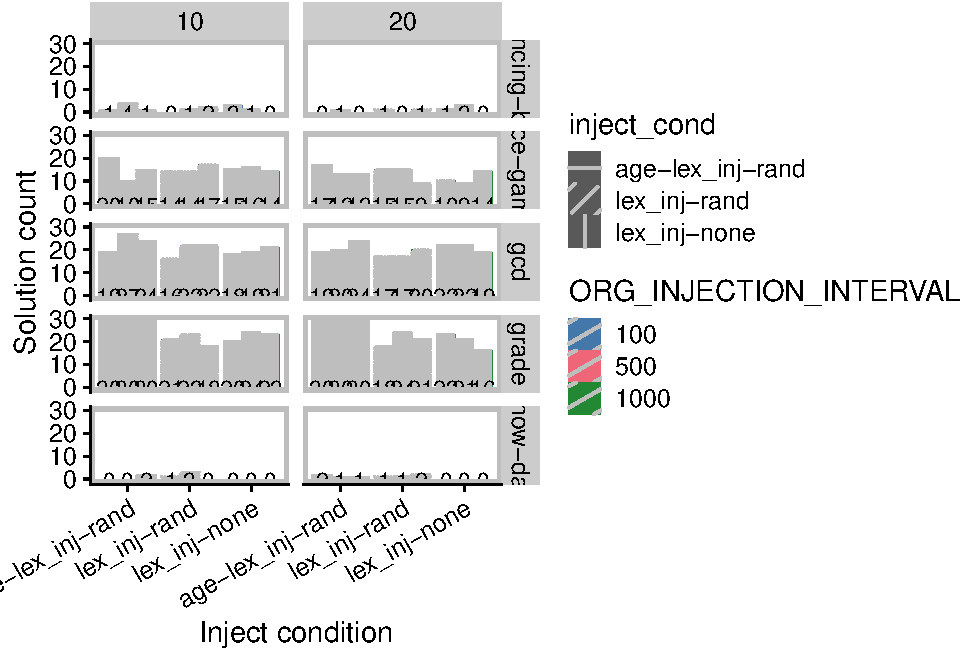
\includegraphics{age-based-lex-supplemental_files/figure-latex/unnamed-chunk-7-1.pdf}

\hypertarget{interval-100-with-age-order-limit-10}{%
\section{Interval 100 with age order limit 10}\label{interval-100-with-age-order-limit-10}}

\hypertarget{problem-solving-success}{%
\subsection{Problem-solving success}\label{problem-solving-success}}

\begin{lstlisting}[language=R]
plot <- solution_counts %>%
  filter(ORG_INJECTION_INTERVAL == "100" & AGE_LEX_AGE_ORDER_LIMIT == "10") %>%
  ggplot(
    aes(
      x = inject_cond,
      y = solution_count,
      fill = inject_cond
    )
  ) +
  geom_col() +
  geom_text(
    aes(y = -0.7, label = solution_count),
    position = position_dodge(width=0.9)
  ) +
  scale_fill_bright() +
  scale_color_bright() +
  scale_x_discrete(
    name = "Inject condition",
    limits = c("age-lex_inj-rand", "lex_inj-rand", "lex_inj-none"),
    labels = c("Random inj.\nAge sel.", "Random inj.\nNo Age", "Standard\nLex.")
  ) +
  scale_y_continuous(
    "Solution count"
  ) +
  facet_wrap(
    ~ PROBLEM,
    nrow = 1
  ) +
  theme(
      legend.position = "none",
      # axis.text.x = element_text(
      #   angle = 30,
      #   hjust = 1
      # ),
      panel.border = element_rect(color = "gray", size = 2)
    )
ggsave(
  filename = paste0(plot_directory, "solutions-bar-i100-ol10.pdf"),
  plot = plot,
  width = 18,
  height = 8
)
plot
\end{lstlisting}

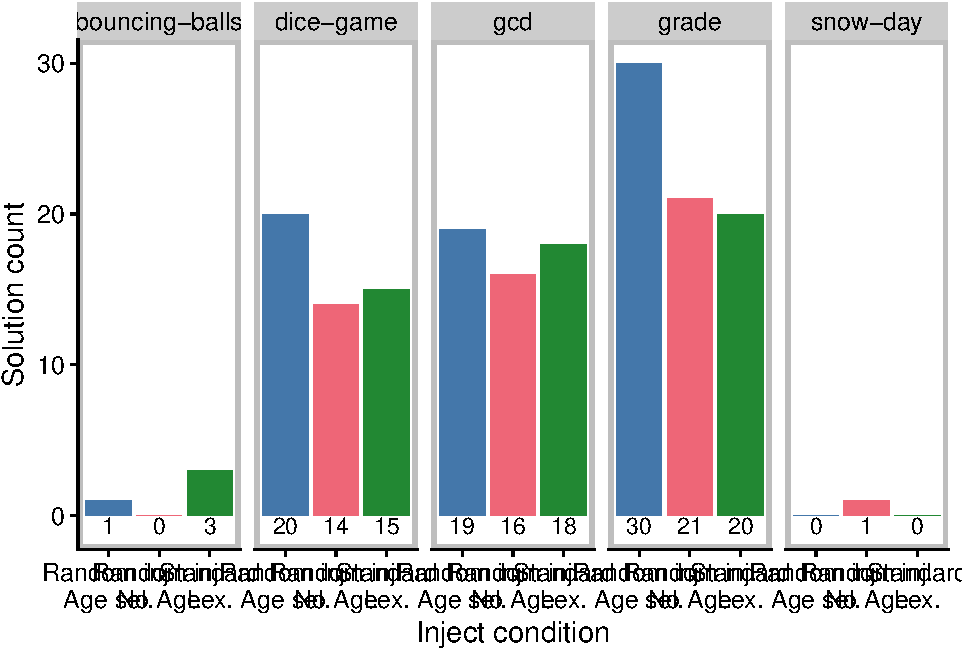
\includegraphics{age-based-lex-supplemental_files/figure-latex/unnamed-chunk-8-1.pdf}

\hypertarget{proportion-of-solutions-that-descend-from-injected-programs}{%
\subsection{Proportion of solutions that descend from injected programs}\label{proportion-of-solutions-that-descend-from-injected-programs}}

\begin{lstlisting}[language=R]
plot <- solution_counts %>%
  filter(ORG_INJECTION_INTERVAL == "100" & AGE_LEX_AGE_ORDER_LIMIT == "10") %>%
  ggplot(
    aes(
      x = inject_cond,
      # y = solution_count,
      y = sol_from_injected,
      fill = inject_cond
    )
  ) +
  geom_col(aes(y = solution_count), fill = "grey", alpha = 0.8) +
  geom_col() +
  geom_text(
    aes(y = -0.7, label = paste0(sol_from_injected, "/", solution_count)),
    position = position_dodge(width=0.9)
  ) +
  scale_fill_bright() +
  scale_color_bright() +
  scale_x_discrete(
    name = "Inject condition",
    limits = c("age-lex_inj-rand", "lex_inj-rand", "lex_inj-none"),
    labels = c("Random inj.\nAge sel.", "Random inj.\nNo Age", "Standard\nLex.")
  ) +
  scale_y_continuous(
    "Solution count"
  ) +
  facet_wrap(
    ~ PROBLEM,
    nrow = 1
  ) +
  theme(
      legend.position = "none",
      # axis.text.x = element_text(
      #   angle = 30,
      #   hjust = 1
      # ),
      panel.border = element_rect(color = "gray", size = 2)
    )
ggsave(
  filename = paste0(plot_directory, "solutions-bar-i100-ol10-prop-descend.pdf"),
  plot = plot,
  width = 18,
  height = 8
)
plot
\end{lstlisting}

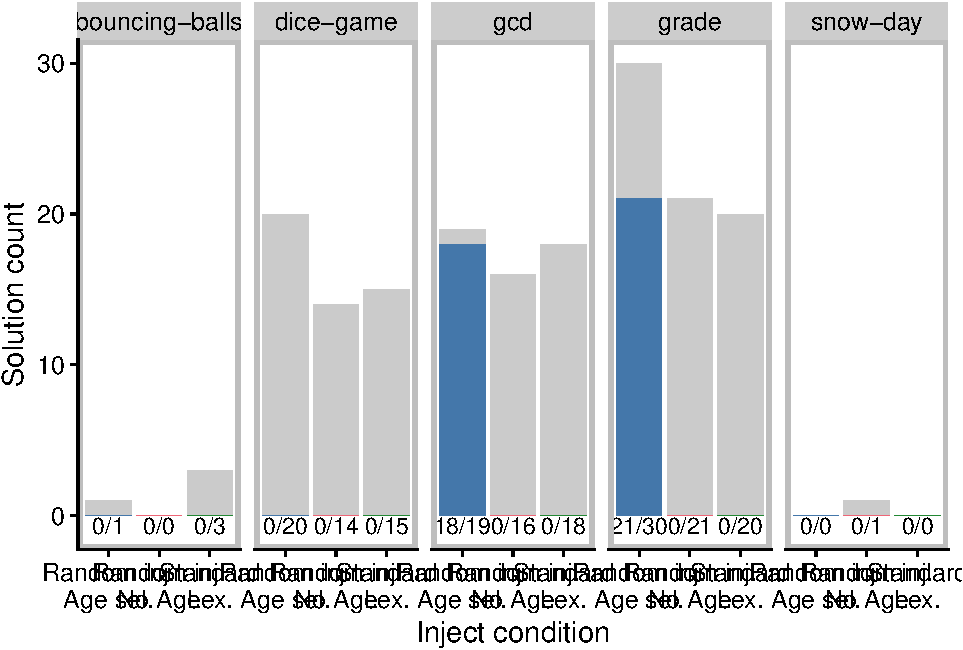
\includegraphics{age-based-lex-supplemental_files/figure-latex/unnamed-chunk-9-1.pdf}

\hypertarget{statistics}{%
\subsubsection{Statistics}\label{statistics}}

\begin{lstlisting}[language=R]
sol_stats_data <- solution_counts %>%
  ungroup() %>%
  select(
    PROBLEM,
    ORG_INJECTION_INTERVAL,
    AGE_LEX_AGE_ORDER_LIMIT,
    inject_cond,
    solution_count,
    no_solution_count
  )

fisher_results <- data.frame(
  comparison = character(),
  group1 = character(),
  group2 = character(),
  n = integer(),
  p = double(),
  p.adj = double(),
  p.adj.signif = character()
)


# ORG_INJECTION_INTERVAL
# AGE_LEX_AGE_ORDER_LIMIT
inj_intervals <- levels(sol_stats_data$ORG_INJECTION_INTERVAL)
age_limits <- levels(sol_stats_data$AGE_LEX_AGE_ORDER_LIMIT)
problems <- levels(sol_stats_data$PROBLEM)

for (inj_interval in inj_intervals) {
  for (age_limit in age_limits) {
    for (problem in problems) {
      ft_results <- sol_stats_data %>%
        filter(
          PROBLEM == problem & AGE_LEX_AGE_ORDER_LIMIT == age_limit & ORG_INJECTION_INTERVAL == inj_interval
        ) %>%
        select(inject_cond, solution_count, no_solution_count) %>%
        column_to_rownames(var = "inject_cond") %>%
        pairwise_fisher_test(
          p.adjust.method = "holm"
        ) %>%
        add_significance("p.adj")

      ft_results <- ft_results %>%
        mutate(
          problem = rep(problem, nrow(ft_results)),
          inj_interval = rep(inj_interval, nrow(ft_results)),
          age_limit = rep(age_limit, nrow(ft_results)),
          .keep = "all"
        ) %>%
        relocate(problem, inj_interval, age_limit)

      fisher_results <- rbind(
        fisher_results,
        ft_results
      )
    }
  }
}

fisher_results <- as.tibble(fisher_results)
\end{lstlisting}

\begin{lstlisting}
## Warning: `as.tibble()` was deprecated in tibble 2.0.0.
## i Please use `as_tibble()` instead.
## i The signature and semantics have changed, see `?as_tibble`.
## This warning is displayed once every 8 hours.
## Call `lifecycle::last_lifecycle_warnings()` to see where this warning was generated.
\end{lstlisting}

\begin{lstlisting}[language=R]
fisher_results <- fisher_results %>%
  mutate(
    # comparison = as.factor(comparison),
    problem = as.factor(problem),
    inj_interval = as.factor(inj_interval),
    age_limit = as.factor(age_limit),
    group1 = as.factor(group1),
    group2 = as.factor(group2),
  ) %>%
  group_by(
    problem
  )

fisher_table <- kbl(fisher_results) %>% kable_styling()
save_kable(fisher_table, paste0(plot_directory, "stats_table.pdf"))
fisher_table
\end{lstlisting}

\begin{table}
\centering
\begin{tabular}[t]{l|l|l|l|l|r|r|r|l}
\hline
problem & inj\_interval & age\_limit & group1 & group2 & n & p & p.adj & p.adj.signif\\
\hline
bouncing-balls & 100 & 10 & age-lex\_inj-rand & lex\_inj-none & 60 & 6.12e-01 & 1.00e+00 & ns\\
\hline
bouncing-balls & 100 & 10 & age-lex\_inj-rand & lex\_inj-rand & 60 & 1.00e+00 & 1.00e+00 & ns\\
\hline
bouncing-balls & 100 & 10 & lex\_inj-none & lex\_inj-rand & 60 & 2.37e-01 & 7.11e-01 & ns\\
\hline
dice-game & 100 & 10 & age-lex\_inj-rand & lex\_inj-none & 60 & 2.95e-01 & 5.90e-01 & ns\\
\hline
dice-game & 100 & 10 & age-lex\_inj-rand & lex\_inj-rand & 60 & 1.92e-01 & 5.76e-01 & ns\\
\hline
dice-game & 100 & 10 & lex\_inj-none & lex\_inj-rand & 60 & 1.00e+00 & 1.00e+00 & ns\\
\hline
gcd & 100 & 10 & age-lex\_inj-rand & lex\_inj-none & 60 & 1.00e+00 & 1.00e+00 & ns\\
\hline
gcd & 100 & 10 & age-lex\_inj-rand & lex\_inj-rand & 60 & 6.01e-01 & 1.00e+00 & ns\\
\hline
gcd & 100 & 10 & lex\_inj-none & lex\_inj-rand & 60 & 7.95e-01 & 1.00e+00 & ns\\
\hline
grade & 100 & 10 & age-lex\_inj-rand & lex\_inj-none & 60 & 7.97e-04 & 2.39e-03 & **\\
\hline
grade & 100 & 10 & age-lex\_inj-rand & lex\_inj-rand & 60 & 1.94e-03 & 3.88e-03 & **\\
\hline
grade & 100 & 10 & lex\_inj-none & lex\_inj-rand & 60 & 1.00e+00 & 1.00e+00 & ns\\
\hline
snow-day & 100 & 10 & age-lex\_inj-rand & lex\_inj-none & 60 & 1.00e+00 & 1.00e+00 & ns\\
\hline
snow-day & 100 & 10 & age-lex\_inj-rand & lex\_inj-rand & 60 & 1.00e+00 & 1.00e+00 & ns\\
\hline
snow-day & 100 & 10 & lex\_inj-none & lex\_inj-rand & 60 & 1.00e+00 & 1.00e+00 & ns\\
\hline
bouncing-balls & 100 & 20 & age-lex\_inj-rand & lex\_inj-none & 60 & 1.00e+00 & 1.00e+00 & ns\\
\hline
bouncing-balls & 100 & 20 & age-lex\_inj-rand & lex\_inj-rand & 60 & 1.00e+00 & 1.00e+00 & ns\\
\hline
bouncing-balls & 100 & 20 & lex\_inj-none & lex\_inj-rand & 60 & 1.00e+00 & 1.00e+00 & ns\\
\hline
dice-game & 100 & 20 & age-lex\_inj-rand & lex\_inj-none & 60 & 1.19e-01 & 3.57e-01 & ns\\
\hline
dice-game & 100 & 20 & age-lex\_inj-rand & lex\_inj-rand & 60 & 7.96e-01 & 7.96e-01 & ns\\
\hline
dice-game & 100 & 20 & lex\_inj-none & lex\_inj-rand & 60 & 2.95e-01 & 5.90e-01 & ns\\
\hline
gcd & 100 & 20 & age-lex\_inj-rand & lex\_inj-none & 60 & 5.80e-01 & 1.00e+00 & ns\\
\hline
gcd & 100 & 20 & age-lex\_inj-rand & lex\_inj-rand & 60 & 7.92e-01 & 1.00e+00 & ns\\
\hline
gcd & 100 & 20 & lex\_inj-none & lex\_inj-rand & 60 & 2.79e-01 & 8.37e-01 & ns\\
\hline
grade & 100 & 20 & age-lex\_inj-rand & lex\_inj-none & 60 & 1.05e-02 & 2.10e-02 & *\\
\hline
grade & 100 & 20 & age-lex\_inj-rand & lex\_inj-rand & 60 & 1.24e-04 & 3.72e-04 & ***\\
\hline
grade & 100 & 20 & lex\_inj-none & lex\_inj-rand & 60 & 2.67e-01 & 2.67e-01 & ns\\
\hline
snow-day & 100 & 20 & age-lex\_inj-rand & lex\_inj-none & 60 & 4.92e-01 & 1.00e+00 & ns\\
\hline
snow-day & 100 & 20 & age-lex\_inj-rand & lex\_inj-rand & 60 & 1.00e+00 & 1.00e+00 & ns\\
\hline
snow-day & 100 & 20 & lex\_inj-none & lex\_inj-rand & 60 & 1.00e+00 & 1.00e+00 & ns\\
\hline
bouncing-balls & 500 & 10 & age-lex\_inj-rand & lex\_inj-none & 60 & 3.53e-01 & 1.00e+00 & ns\\
\hline
bouncing-balls & 500 & 10 & age-lex\_inj-rand & lex\_inj-rand & 60 & 3.53e-01 & 1.00e+00 & ns\\
\hline
bouncing-balls & 500 & 10 & lex\_inj-none & lex\_inj-rand & 60 & 1.00e+00 & 1.00e+00 & ns\\
\hline
dice-game & 500 & 10 & age-lex\_inj-rand & lex\_inj-none & 60 & 1.92e-01 & 5.76e-01 & ns\\
\hline
dice-game & 500 & 10 & age-lex\_inj-rand & lex\_inj-rand & 60 & 4.30e-01 & 8.60e-01 & ns\\
\hline
dice-game & 500 & 10 & lex\_inj-none & lex\_inj-rand & 60 & 7.97e-01 & 8.60e-01 & ns\\
\hline
gcd & 500 & 10 & age-lex\_inj-rand & lex\_inj-none & 60 & 3.03e-02 & 9.09e-02 & ns\\
\hline
gcd & 500 & 10 & age-lex\_inj-rand & lex\_inj-rand & 60 & 1.81e-01 & 3.62e-01 & ns\\
\hline
gcd & 500 & 10 & lex\_inj-none & lex\_inj-rand & 60 & 5.80e-01 & 5.80e-01 & ns\\
\hline
grade & 500 & 10 & age-lex\_inj-rand & lex\_inj-none & 60 & 2.37e-02 & 4.74e-02 & *\\
\hline
grade & 500 & 10 & age-lex\_inj-rand & lex\_inj-rand & 60 & 1.05e-02 & 3.15e-02 & *\\
\hline
grade & 500 & 10 & lex\_inj-none & lex\_inj-rand & 60 & 1.00e+00 & 1.00e+00 & ns\\
\hline
snow-day & 500 & 10 & age-lex\_inj-rand & lex\_inj-none & 60 & 1.00e+00 & 1.00e+00 & ns\\
\hline
snow-day & 500 & 10 & age-lex\_inj-rand & lex\_inj-rand & 60 & 2.37e-01 & 7.11e-01 & ns\\
\hline
snow-day & 500 & 10 & lex\_inj-none & lex\_inj-rand & 60 & 2.37e-01 & 7.11e-01 & ns\\
\hline
bouncing-balls & 500 & 20 & age-lex\_inj-rand & lex\_inj-none & 60 & 6.12e-01 & 1.00e+00 & ns\\
\hline
bouncing-balls & 500 & 20 & age-lex\_inj-rand & lex\_inj-rand & 60 & 1.00e+00 & 1.00e+00 & ns\\
\hline
bouncing-balls & 500 & 20 & lex\_inj-none & lex\_inj-rand & 60 & 2.37e-01 & 7.11e-01 & ns\\
\hline
dice-game & 500 & 20 & age-lex\_inj-rand & lex\_inj-none & 60 & 4.22e-01 & 8.44e-01 & ns\\
\hline
dice-game & 500 & 20 & age-lex\_inj-rand & lex\_inj-rand & 60 & 7.96e-01 & 8.44e-01 & ns\\
\hline
dice-game & 500 & 20 & lex\_inj-none & lex\_inj-rand & 60 & 1.87e-01 & 5.61e-01 & ns\\
\hline
gcd & 500 & 20 & age-lex\_inj-rand & lex\_inj-none & 60 & 7.79e-01 & 1.00e+00 & ns\\
\hline
gcd & 500 & 20 & age-lex\_inj-rand & lex\_inj-rand & 60 & 5.96e-01 & 1.00e+00 & ns\\
\hline
gcd & 500 & 20 & lex\_inj-none & lex\_inj-rand & 60 & 2.79e-01 & 8.37e-01 & ns\\
\hline
grade & 500 & 20 & age-lex\_inj-rand & lex\_inj-none & 60 & 1.94e-03 & 5.82e-03 & **\\
\hline
grade & 500 & 20 & age-lex\_inj-rand & lex\_inj-rand & 60 & 2.37e-02 & 4.74e-02 & *\\
\hline
grade & 500 & 20 & lex\_inj-none & lex\_inj-rand & 60 & 5.52e-01 & 5.52e-01 & ns\\
\hline
snow-day & 500 & 20 & age-lex\_inj-rand & lex\_inj-none & 60 & 1.00e+00 & 1.00e+00 & ns\\
\hline
snow-day & 500 & 20 & age-lex\_inj-rand & lex\_inj-rand & 60 & 1.00e+00 & 1.00e+00 & ns\\
\hline
snow-day & 500 & 20 & lex\_inj-none & lex\_inj-rand & 60 & 1.00e+00 & 1.00e+00 & ns\\
\hline
bouncing-balls & 1000 & 10 & age-lex\_inj-rand & lex\_inj-none & 60 & 1.00e+00 & 1.00e+00 & ns\\
\hline
bouncing-balls & 1000 & 10 & age-lex\_inj-rand & lex\_inj-rand & 60 & 1.00e+00 & 1.00e+00 & ns\\
\hline
bouncing-balls & 1000 & 10 & lex\_inj-none & lex\_inj-rand & 60 & 4.92e-01 & 1.00e+00 & ns\\
\hline
dice-game & 1000 & 10 & age-lex\_inj-rand & lex\_inj-none & 60 & 1.00e+00 & 1.00e+00 & ns\\
\hline
dice-game & 1000 & 10 & age-lex\_inj-rand & lex\_inj-rand & 60 & 7.96e-01 & 1.00e+00 & ns\\
\hline
dice-game & 1000 & 10 & lex\_inj-none & lex\_inj-rand & 60 & 6.06e-01 & 1.00e+00 & ns\\
\hline
gcd & 1000 & 10 & age-lex\_inj-rand & lex\_inj-none & 60 & 5.52e-01 & 1.00e+00 & ns\\
\hline
gcd & 1000 & 10 & age-lex\_inj-rand & lex\_inj-rand & 60 & 7.61e-01 & 1.00e+00 & ns\\
\hline
gcd & 1000 & 10 & lex\_inj-none & lex\_inj-rand & 60 & 1.00e+00 & 1.00e+00 & ns\\
\hline
grade & 1000 & 10 & age-lex\_inj-rand & lex\_inj-none & 60 & 1.05e-02 & 2.10e-02 & *\\
\hline
grade & 1000 & 10 & age-lex\_inj-rand & lex\_inj-rand & 60 & 1.24e-04 & 3.72e-04 & ***\\
\hline
grade & 1000 & 10 & lex\_inj-none & lex\_inj-rand & 60 & 2.67e-01 & 2.67e-01 & ns\\
\hline
snow-day & 1000 & 10 & age-lex\_inj-rand & lex\_inj-none & 60 & 4.92e-01 & 1.00e+00 & ns\\
\hline
snow-day & 1000 & 10 & age-lex\_inj-rand & lex\_inj-rand & 60 & 4.92e-01 & 1.00e+00 & ns\\
\hline
snow-day & 1000 & 10 & lex\_inj-none & lex\_inj-rand & 60 & 1.00e+00 & 1.00e+00 & ns\\
\hline
bouncing-balls & 1000 & 20 & age-lex\_inj-rand & lex\_inj-none & 60 & 1.00e+00 & 1.00e+00 & ns\\
\hline
bouncing-balls & 1000 & 20 & age-lex\_inj-rand & lex\_inj-rand & 60 & 1.00e+00 & 1.00e+00 & ns\\
\hline
bouncing-balls & 1000 & 20 & lex\_inj-none & lex\_inj-rand & 60 & 1.00e+00 & 1.00e+00 & ns\\
\hline
dice-game & 1000 & 20 & age-lex\_inj-rand & lex\_inj-none & 60 & 1.00e+00 & 1.00e+00 & ns\\
\hline
dice-game & 1000 & 20 & age-lex\_inj-rand & lex\_inj-rand & 60 & 4.22e-01 & 8.64e-01 & ns\\
\hline
dice-game & 1000 & 20 & lex\_inj-none & lex\_inj-rand & 60 & 2.88e-01 & 8.64e-01 & ns\\
\hline
gcd & 1000 & 20 & age-lex\_inj-rand & lex\_inj-none & 60 & 2.52e-01 & 7.56e-01 & ns\\
\hline
gcd & 1000 & 20 & age-lex\_inj-rand & lex\_inj-rand & 60 & 3.82e-01 & 7.64e-01 & ns\\
\hline
gcd & 1000 & 20 & lex\_inj-none & lex\_inj-rand & 60 & 1.00e+00 & 1.00e+00 & ns\\
\hline
grade & 1000 & 20 & age-lex\_inj-rand & lex\_inj-none & 60 & 1.68e-05 & 5.04e-05 & ****\\
\hline
grade & 1000 & 20 & age-lex\_inj-rand & lex\_inj-rand & 60 & 1.94e-03 & 3.88e-03 & **\\
\hline
grade & 1000 & 20 & lex\_inj-none & lex\_inj-rand & 60 & 2.88e-01 & 2.88e-01 & ns\\
\hline
snow-day & 1000 & 20 & age-lex\_inj-rand & lex\_inj-none & 60 & 1.00e+00 & 1.00e+00 & ns\\
\hline
snow-day & 1000 & 20 & age-lex\_inj-rand & lex\_inj-rand & 60 & 1.00e+00 & 1.00e+00 & ns\\
\hline
snow-day & 1000 & 20 & lex\_inj-none & lex\_inj-rand & 60 & 4.92e-01 & 1.00e+00 & ns\\
\hline
\end{tabular}
\end{table}

  \bibliography{packages.bib,supplemental.bib}

\end{document}
